%!TEX root = ../main.tex
%%%%%%%%%%%%%%%%%%%%%%%%%%%%%%%%%%
% Links:
%
% Difficulty:
% Companies: 
%%%%%%%%%%%%%%%%%%%%%%%%%%%%%%%%%%

\chapter{Generate points in circle uniformly}
\label{ch:random_points_in_circle}
\section*{Introduction}
The problem described in this Chapter is about generating a (possibly large) number of random points in a circle of a certain radius. Said points need to be generated uniformly. Despite its simplicity the problem still poses some unexpected challenges and difficulties. We will discuss how to approach this problem and also one solution that many candidates provides and that seems just correct but that should absolutely be avoided as it is not correct (spoiler it does not distribute points uniformly). We will also look at some cool figures or points in a circle.

\section{Problem statement}
\begin{exercise}
Write a function that, given a circle of radius $r$ and centered at $(x,y)$ where $r,x,y \in \mathcal{R}$ returns a uniformly distributed point in the circle.
\end{exercise}



\begin{example}
	\hfill \\

	
\end{example}

\section{Clarification Questions}

\begin{QandA}
	\item What does really mean for the point to be uniformly distributed?
	\begin{answered}
		\textit{It means that every point of the circle has the same probability of being picked/generated by the function}
	\end{answered}
\end{QandA}

\section{Discussion}
\label{random_points_in_circle:sec:discussion}

\subsubsection{Wrong approach}
\label{random_points_in_circle:sec:buggy}
Let's start by discussing a common approach that comes naturally to mind. One might think that in order to pick a point in the circle is it sufficient to 
\begin{enumerate}
	\item Pick a random angle $\theta \in [0, 2\pi[ $
	\item Pick a random radius $\overline{r} \in [0,r]$
	\item Generate the Cartesian coordinates of the point given the radius and the angle (polar coordinates \cite{cit:wiki:polar_coordinates}) as (see Figure \ref{fig:random_points_in_cirle:polar_coordinates}):
	\begin{gather*}
		 x=\overline{r}\sin(\theta) \\
		 y=\overline{r}\cos(\theta) 
	\end{gather*}
\end{enumerate}

\begin{figure}
	\label{fig:random_points_in_cirle:polar_coordinates}
	\centering
	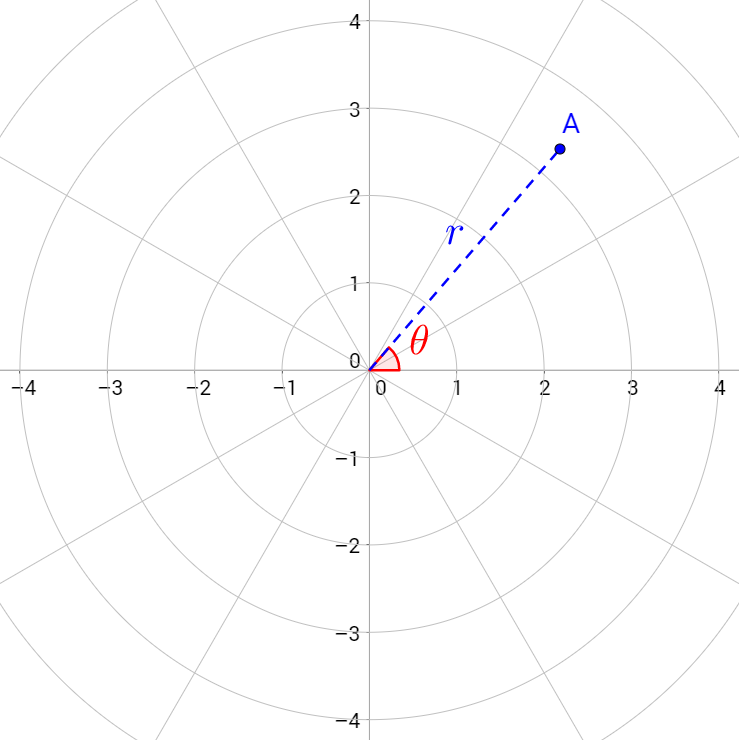
\includegraphics[scale=0.3]{sources/random_points_in_circle/images/polar-coordinate}
	\caption{Generation of a random point in polar coordinates given a random angle $\theta$ and a random radius $r$.}
\end{figure}

Despite its simplicity this approach is wrong as it does not produce points uniformly distributed in the circle? Before having a quick look at the proof it is instructive to have a look Figure \ref{fig:random_points_in_cirle:buggy} which is drawing a large number of points on the circle generated using this buggy solution. As you can see the points are not generated uniformly as their density is higher towards the center. 

\begin{figure}
	\label{fig:random_points_in_cirle:buggy}
	\centering
	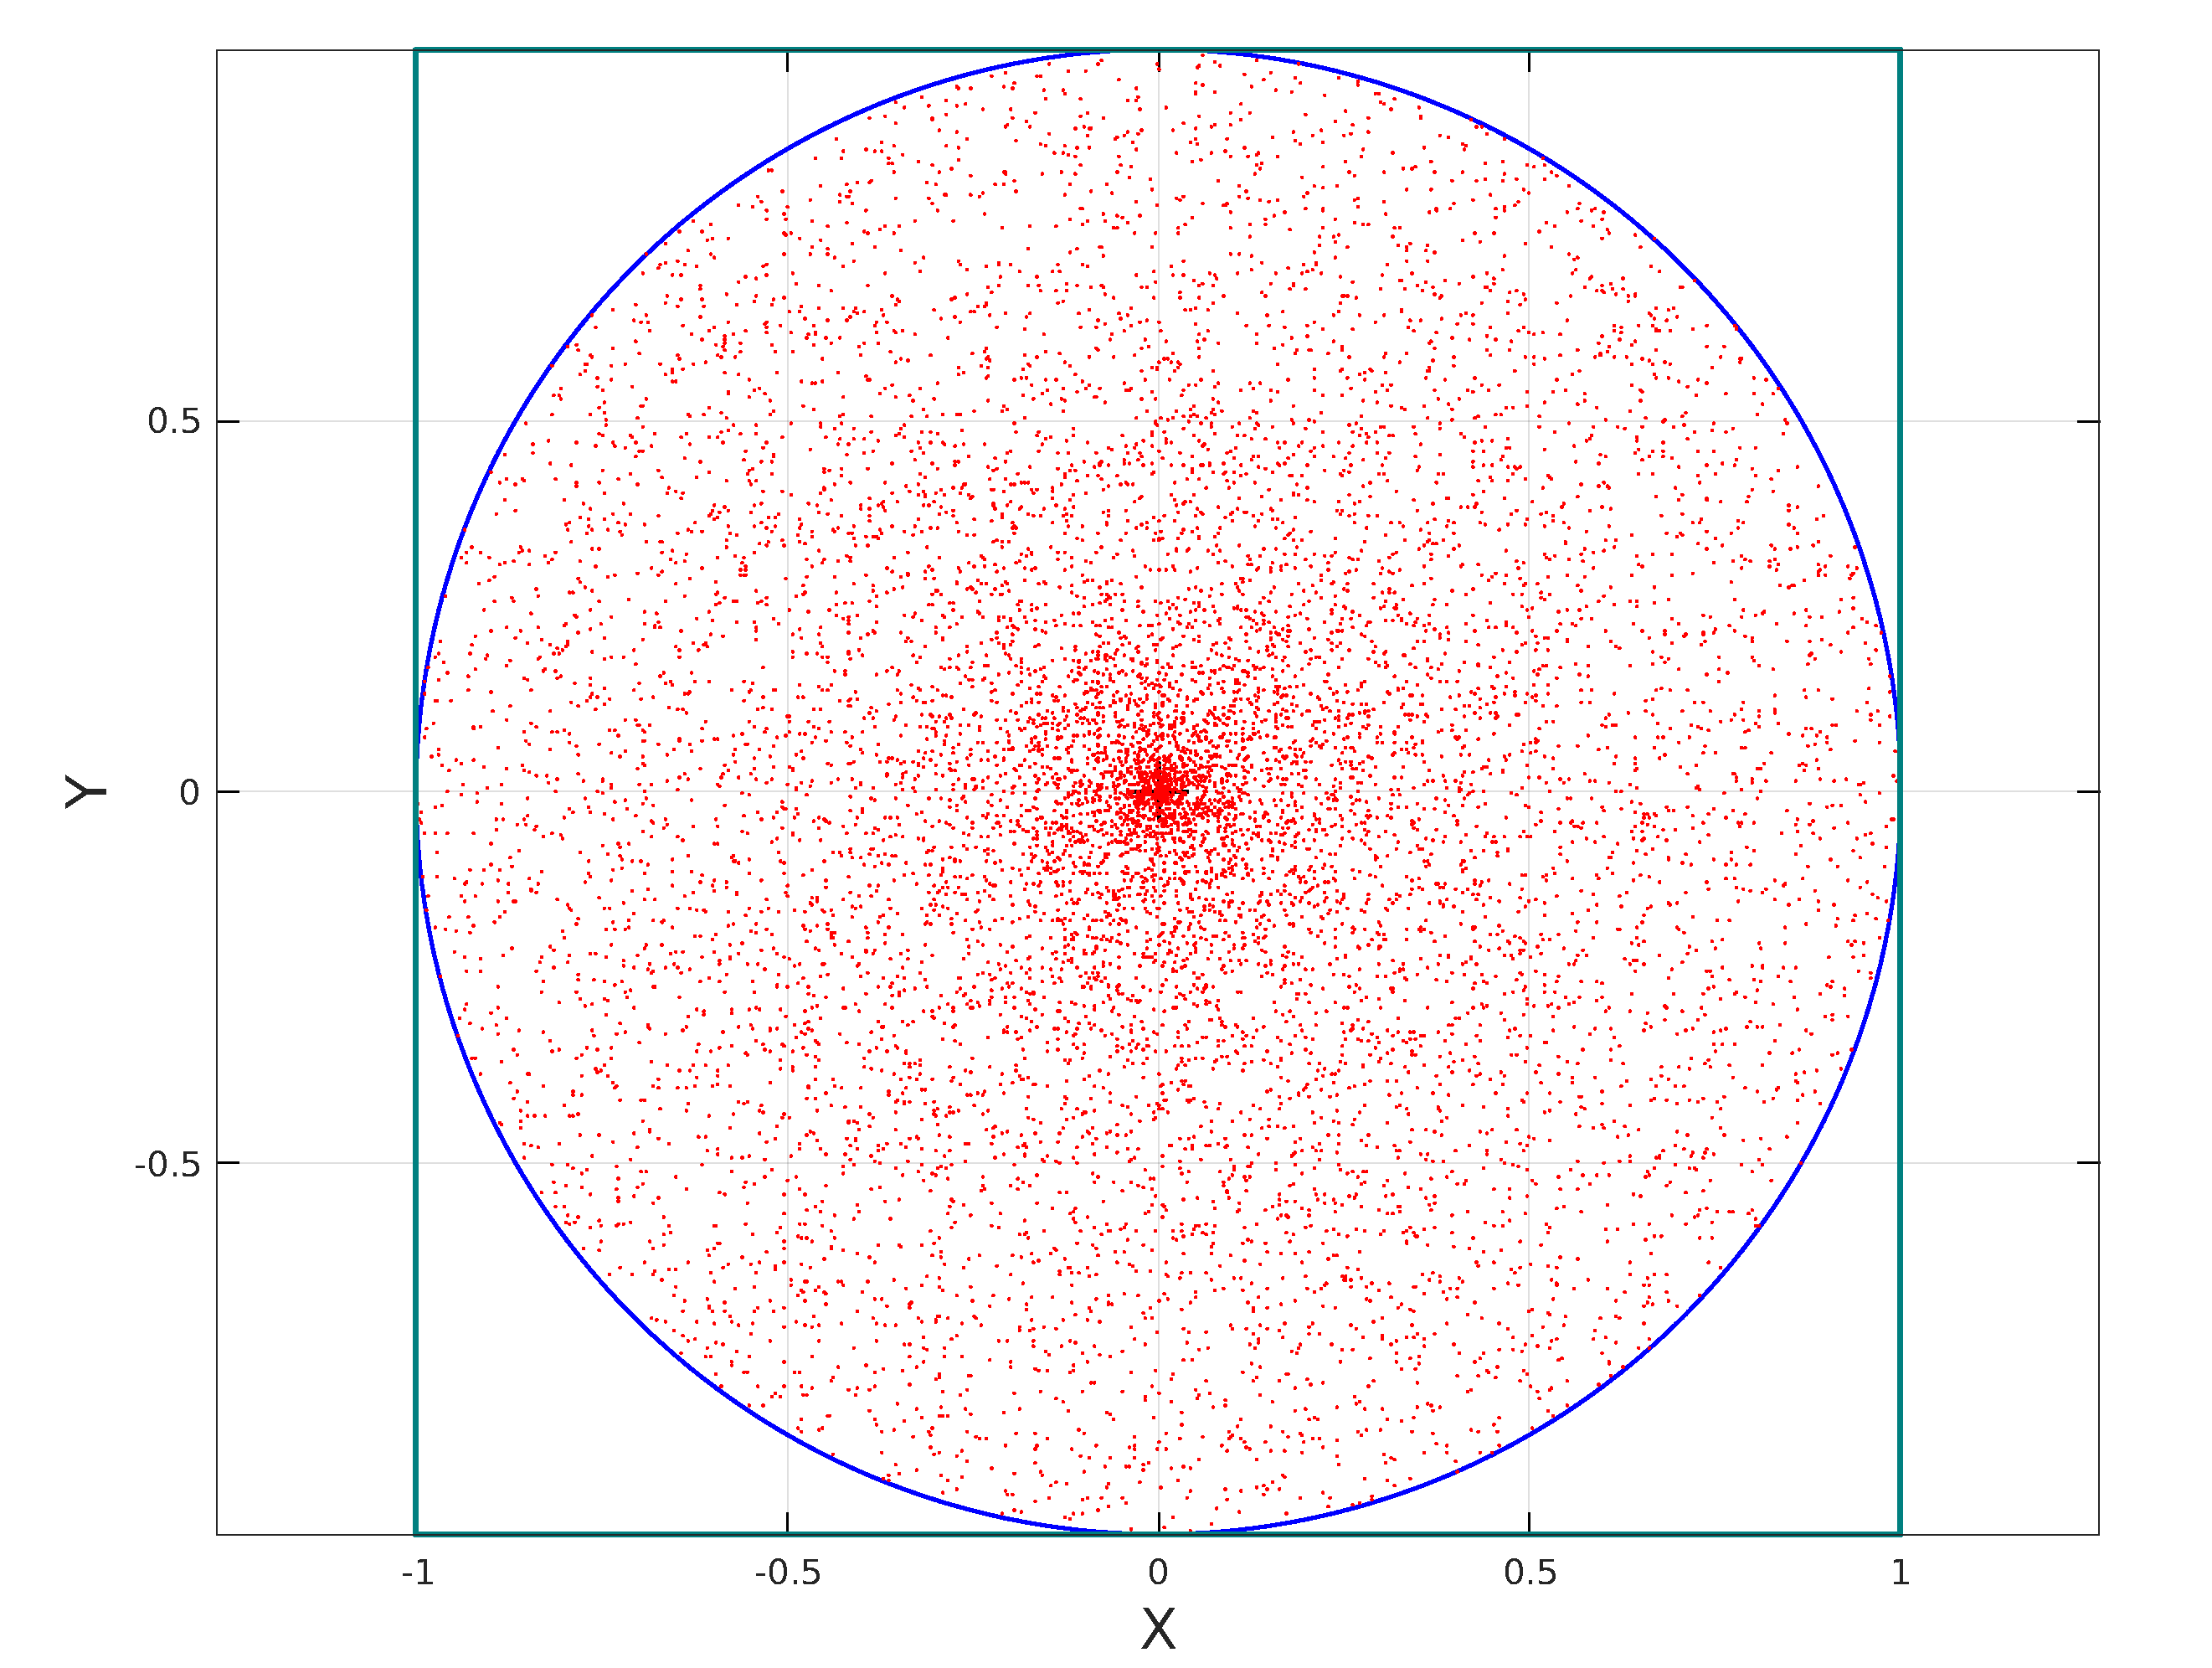
\includegraphics[scale=0.3]{sources/random_points_in_circle/images/buggy_points}
	\caption{Large number of points generated using the approach described in Section \ref{random_points_in_circle:sec:buggy}.}
\end{figure}

\subsubsection{Loop approach}
\label{random_points_in_circle:sec:loop}

\begin{figure}
	\label{fig:random_points_in_cirle:loop}
	\centering
	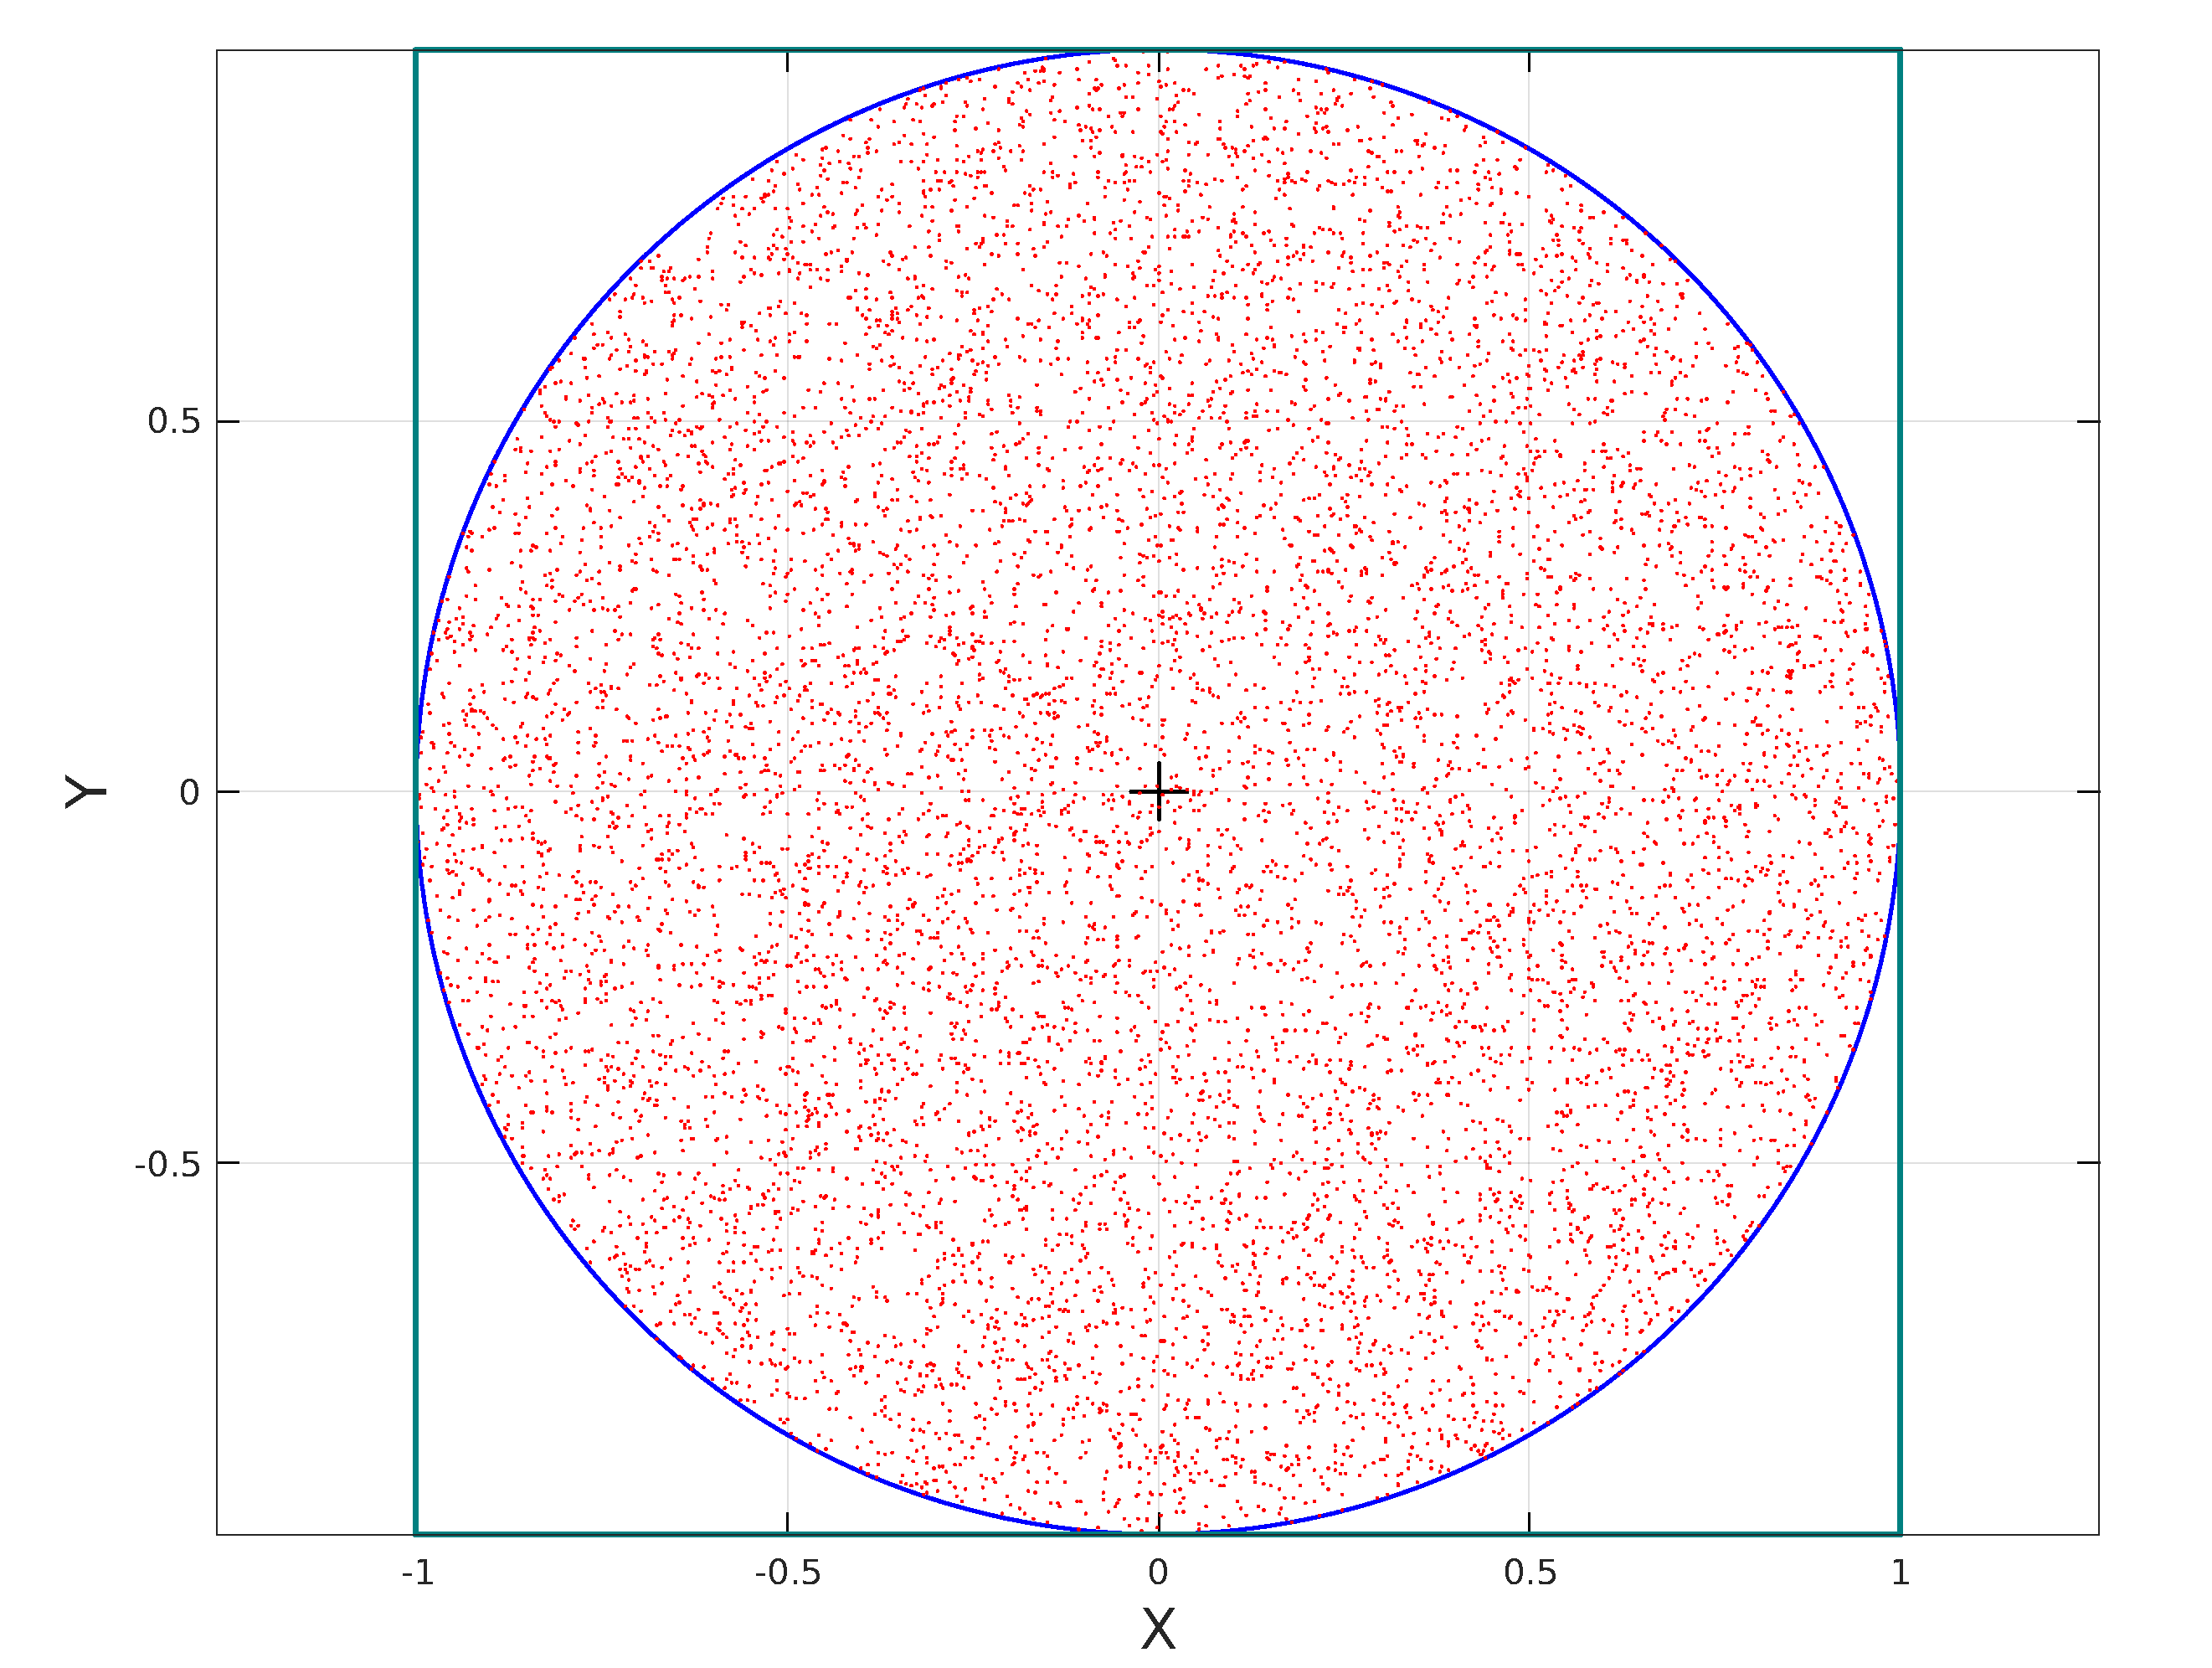
\includegraphics[scale=0.3]{sources/random_points_in_circle/images/loop_points}
	\caption{Large number of points generated using the approach described in Section \ref{random_points_in_circle:sec:loop}.}
\end{figure}

\subsection{Brute-force}
\label{random_points_in_circle:sec:bruteforce}

\lstinputlisting[language=c++, caption=Sample Caption,label=list:random_points_in_circle]{sources/random_points_in_circle/random_points_in_circle_solution1.cpp}

